\section{Evaluation}
\label{sec:evaluation}
For evaluation of the model that is described in section \ref{sec:model} the tool \textit{Tensorboard} is used. This is a suite of visualization tools that can be used to understand, debug and optimize \textit{TensorFlow} programs. In the context of evaluation, \textit{Tensorboard} is used to visualize the 
\begin{itemize}
	\item accuracy,
	\item loss and
	\item graph
\end{itemize}
of the model. As validation technique the k fold cross validation is being deployed. How this technique works and how it is integrated within the architecture is described in the subsection \ref{subsec:kfoldxvalidation}. In \ref{subsec:xvalidationresults} the yielded results of this technique are explained. Finally, the trained model and an unused dataset are used to predict the rising or falling of the contained stocks. In \ref{subsec:predresults} the outcome of this validation of the model against to this point unknown data to the model is presented. 

\subsection{K fold cross validation}
\label{subsec:kfoldxvalidation}
The most simple method for cross validation is the \textit{holdout} method. This technique splits the available dataset into two distinct sets - training and validation. In terms of variance this method is disadvantageous as it is not certain which data points end up in the validation set. This can lead to losing important patterns during training and, therefore, underfitting. 
\\
The technique of k fold cross validation provides a method of using the available data efficiently for training as well as validation. The data is split into $k$ subsets and the \textit{holdout} method is applied $k$ times to these sets. In each iteration a different set of the $k$ datasets is used as validation set and the remaining $k-1$ sets are used for training. As a result, each data point is used multiple times for training at some point in the loop and once for validation. Consequently, most of the data is used for fitting so that the bias is greatly reduced and by using most data for validation this also reduces the variance. The swap of training and validation data for each iteration also contributes to the efficiency of this technique. 
\\
The evaluation of the model by the k fold cross validation is achieved by logging the accuracy and loss. Those two scalars are measured for every iteration during the cross validation and after the $k$ iterations for the current epoch. During each of the $k$ iterations the mean of the accuracy and loss for all batches is calculated and written to a \textit{Tensorboard} chart. After the $k$ iterations the mean of all previously calculated average accuracies and losses is determined and also written to a \textit{Tensorboard} chart, whereas the x-axis displays the epoch of this result. The calculation for those mean values is done outside the \textit{TensorFlow} graph. Although this is not best practice, the mean calculation for those scalars would have been quite challenging to do inside the graph as a definition for the epoch is not possible at the level of graph definition. 

\subsection{Results of the cross validation}
\label{subsec:xvalidationresults}
k fold cross validation as described in \ref{subsec:kfoldxvalidation}, logged final scalar result over all epochs
\begin{figure}[!ht]
	\caption{A Graph depicting the mean accuracy over 650 epochs of the k fold cross validation with $k=10$. Also, dropout was being used with a probability of 0.3. }
	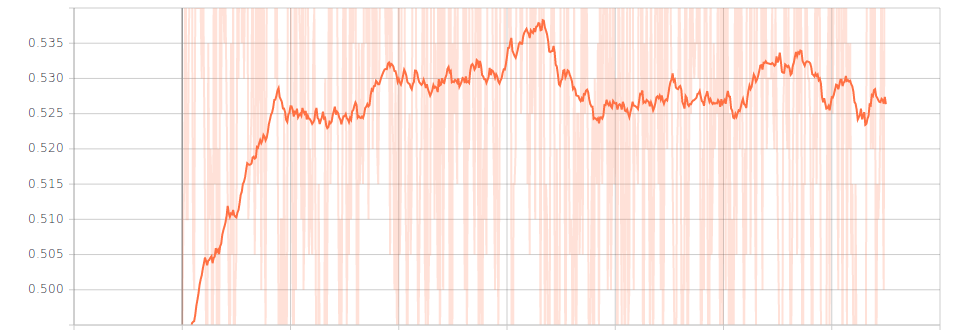
\includegraphics[width=0.95\linewidth]{images/evaluation/650-epochs-k-crossvalidation-accuracy-mean.png}
	\label{fig:acc650epochs}
\end{figure}
\begin{figure}[!ht]
	\caption{A Graph depicting the mean loss over 650 epochs of the k fold cross validation with $k=10$. Also, dropout was being used with a probability of 0.3. }
	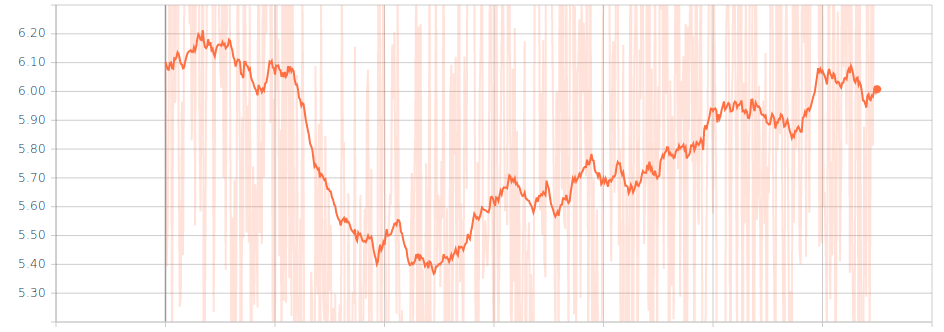
\includegraphics[width=0.95\linewidth]{images/evaluation/650-epochs-k-crossvalidation-loss-mean.png}
	\label{fig:loss650epochs}
\end{figure}

\subsection{Prediction results}
\label{subsec:predresults}
TODO: Daniel